\chapter{Network Traffic Simulator:  Structure and Architecture}
\label{Structure}

\par This software is comprised of several interconnected modules.  Each module represents an abstract concept required for modelling a traffic scenario, each containing as many classes as are needed to create the components necessarily for that concept.  This results in the creation of three self\-contained modules representing the network, the cars/objects traversing the network, and the state-changer.  To make the simulation complete and fully self-contained, the user may utilize two additional optional modules for generating the network structure and car objects. Following naming conventions, and module that a user may directly interact with has been named using capitalization; dependent modules (hidden to the user) are named using only lowercase.

\section{Essential Modules for the Network Traffic \\ Simulator}

\subsection{Network Module:  traffic\_network}

\par As noted in the previous chapter, a network must have three components (network structure, nodes, and edges) \textit{and} there exists an inherent hierarchy to these structures (a network only exists by defining sets of connected nodes).  Though for creation purposes it may make sense to define the nodes and edges and let the network be a dependent object, that does not make sense for the problem at hand:  traffic simulation is the analysis of objects moving over a network, therefore the Network itself must be given (requiring a class of its own), leading to Nodes and Edges being dependent classes.  The module \textbf{traffic\_network} has been created to collect the instances and interactions of all network components for a simulation instance.  \\

\par The resulting module structure is as follows:

\begin{figure}[H]
    \centering
	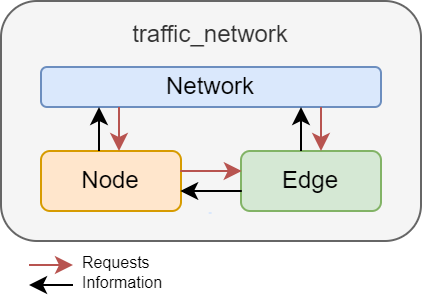
\includegraphics[width=0.5\textwidth]{tex files/Figures/traffic_network_module.png}
	\caption[Network Module:  traffic\_network]{Hierarchical structure of classes within the traffic\_network module.  Directions of requests and information flow between classes is depicted by colored arrows }
	\label{fig:network_module}
\end{figure}


\subsection{Car Module:  network\_cars}

\par "Car" is the general term I use to describe an object traversing the network as it allows for intuitive labeling of its attributes.  Once instantiated, a car is not dependent on the network to continue existing; to represent this semi-independence, the Car class was moved to a separate module:

\begin{figure}[H]
    \centering
	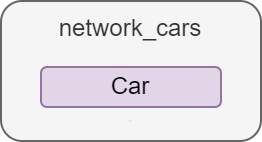
\includegraphics[width=0.3\textwidth]{tex files/Figures/car_module.png}
	\caption[Car Module:  network\_cars]{Classes structure within the network\_cars module}
	\label{fig:cars_module}
\end{figure}

\par In practice, though, the car is not very interesting when trying to simulate overall network behavior and ensuing traffic scenarios.  Any attributes the user may care about (such as current location) are only relevant in context.  So while \textbf{network\_cars} technically exists as a self-contained module, it is never used in isolation.  Instead, this module is automatically imported into the \textbf{traffic\_network} module, seamlessly allowing these two modules to interact with one another.


\subsection{State Module:  Traffic}

\par The final component necessary to creating a simulation  is a mechanism for advancing the state of the network.  State changing includes adding, removing, and advancing any cars on the network as far as possible within a particular unit of time, and are all essential for creating a hands-off simulation. \\

\par But simulation state refers to more than the set of current car locations.  It includes system metadata (like lists of nodes and edges in a network, and their attributes) and dependent calculations from that metadata.  By allowing the user an access point to adapt any component of the network, this software achieves its goal of being adaptable and extensible to other types of networks and simulations.  \\

\par The Traffic modules serves as an API to the underlying simulation, allowing users to (indirectly) interact with the network components and car objects.  The set of all these access points into the simulation allows for the direct management of traffic and has thus been wrapped into an aptly named class,  \textbf{TrafficManager}:

\begin{figure}[H]
    \centering
	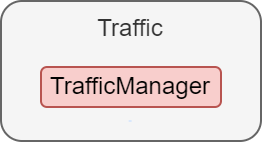
\includegraphics[width=0.3\textwidth]{tex files/Figures/traffic_manager_module.png}
	\caption[State Module:  Traffic\_cars]{Classes structure within the Traffic module}
	\label{fig:traffic_module}
\end{figure}


\noindent  Note that the \textbf{Traffic} module allows only for indirect access to the simulation components.  By using this API as an intermediary between users and network simulation components, the user is given access only to commands that are relevant to analysis, and hide internal functions that facilitate those actions.  For example, if a user wants a particular car to halt in place, they can call on the API function that requests it.  The \textbf{Traffic} module then passes that request to the \textbf{traffic\_network} and/or \textbf{network\_cars} module to handle if and when it becomes relevant.


\section{Essential Module Interaction}

\par Putting the modules together, we get the following depiction of how the modules interact with one another:

\begin{figure}[H]
    \centering
	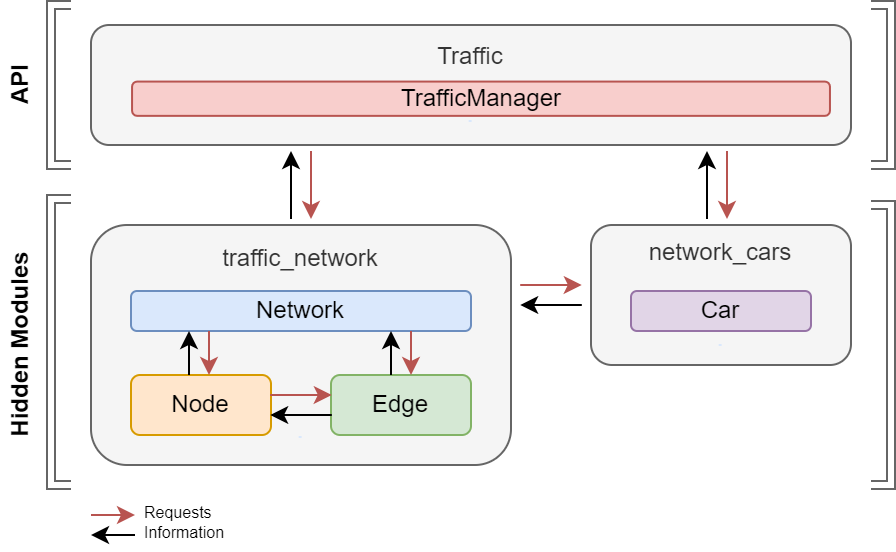
\includegraphics[width=0.9\textwidth]{tex files/Figures/detailed_essentials.png}
	\caption[Software Interaction:  Full View]{Full view of interactions between the modules and their individual components}
	\label{fig:interactions_detailed}
\end{figure}

\noindent  However, as the user doesn't need to concern themselves with the specifics on which functions in which classes work and when, we can streamline the architecture diagram to:

\begin{figure}[H]
    \centering
	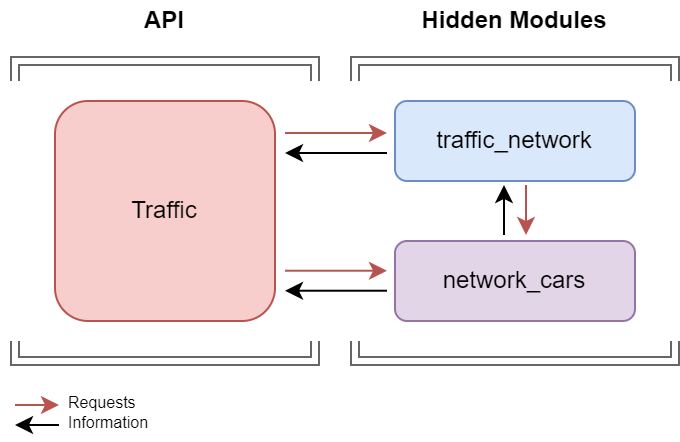
\includegraphics[width=0.7\textwidth]{tex files/Figures/simplified_essentials.png}
	\caption[Software Interaction:  User View]{Generalized overview of interactions between modules}
	\label{fig:interactions_simplified}
\end{figure}



\section{Extended Module Interaction}

\par For the simulation to run, it must be provided with car objects to move on the network and a network object to move the cars along.  How this information is provided to the Traffic module is left up to the user, but some suggestions are provided below.

\subsection{Importing Cars}

\par With existing traffic data, one may want to create a realistic simulation by generating cars and adding them to the network in a way that emulates the real-world data.  To do this, my colleague has created a separate \textbf{CarGenerator} module that allows users to generate cars probabilistically.  This optional module can be run on its own, or integrated directly into the simulation by passing along the \textbf{TrafficManager} and \textbf{Network} instance pointers to the generator.  The details of the generation process and types of patterns the module generates can be found in my colleague's project writeup. \\

\par In lieu of using the \textbf{CarGenerator} module, users may provide their own custom car objects (as a dictionary) as input into the \textbf{TrafficManager} instanciation.  By allowing file-import flexibility to the car adding mechanism, the simulation is therefore capable of using its own snapshot outputs as input to a new simulation.  This allows users to run the same batch of cars (created manually, or by the module) to be run over multiple simulations and compare outputs.



\subsection{Importing a Network}

\par Much like importing cars, flexibility has been given in how network structures can be loaded into the simulation.  \\

\par I have written an optional module, \textbf{UnderlyingNetworkGenerator},  for creating networks based on mathematical concepts like Erdős-Renyi random networks or complete bidirectional networks.  This module creates a stripped-down version of a \textbf{Network} object, assigning only the most essential attributes to individual nodes and edges.  Simple underlying networks may be beneficial for simulations where emphasis is to be placed on the mechanisms of the network action itself (like stoplight cycles or road capacity metering) rather than microscopic analysis.  Though the current version of this module is quite bare-bones, it can (and will) be easily adapted to include more complex, probabilistic attribute assignments. \\

\par For real-world simulations, though, a user would probably prefer to import existing road or network data.  This can be done by converting geojson/csv/shp files to the json format seen in the simulation repository's file "\textit{EXAMPLE\_network\_config.json}".  This method has been tested and confirmed by taking road and waterways WFS data from Het Nationaal Wegenbestand \cite{NWB22} and stripping the "road" segments to just their ID, start-point identifier, end-point identifier, and directionality (if a segment was labeled as bi-directional, then the segment was duplicated with a new ID, reversing the start and end points).


\subsection{Complete Module Interaction}

\par Incorporating the car and network imports and user direction into the Simulation ecosystem, we end up with the resulting User-Software Architecture Model:

\begin{figure}[H]
    \centering
	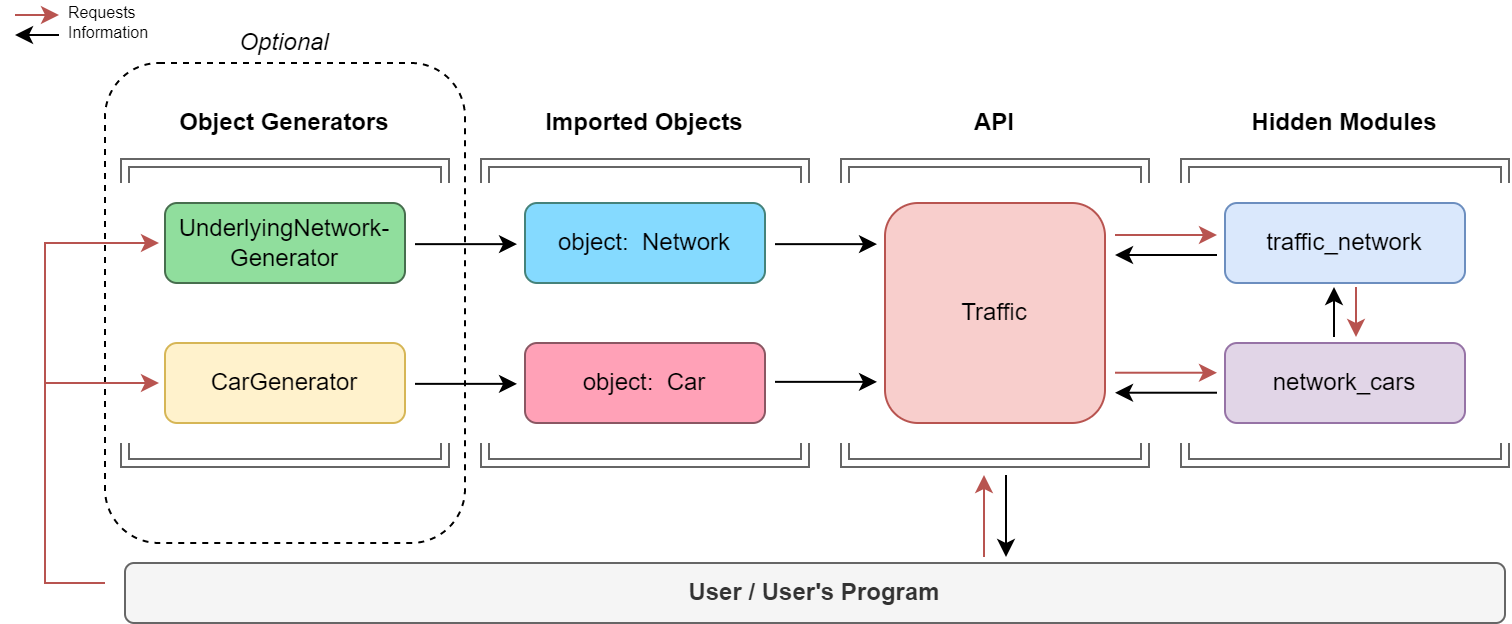
\includegraphics[width=\textwidth]{tex files/Figures/complete_architecture.png}
	\caption[User-Software Interaction]{Generalized overview of interactions between modules, including the use of optional generator modules and/or load files}
	\label{fig:modules_all}
\end{figure}


% \usetikzlibrary{positioning,matrix,shapes.arrows}

% \tikzset{
%   modulematrix/.style={draw=blue!50!red,rounded corners,matrix of nodes,row sep=1cm,column sep=1cm,nodes={draw=green!70,align=center,font=\sffamily},inner ysep=0.5cm},
%   module/.style={rounded corners, align=center, font=\sffamily, thick},
%   simple module/.style={module, top color=blue!10, bottom color=blue!35, draw=blue!75, text width=40mm, minimum height=15mm},
%   module down arrow/.style={module arrow, shape border rotate=-90},
%   module right arrow/.style={module arrow},
% module arrow/.style={single arrow, single arrow head extend=2.5mm, draw=gray!75, inner color=gray!20, outer color=gray!35, thick, shape border uses incircle, anchor=tail,minimum height=0.7cm},
% }

% \begin{tikzpicture}
% \node [simple module] (mA) {Item-1};
% \matrix[modulematrix,below=of mA,label={[anchor=south]below:Item-2}] (mB) {Item-3 & Item-4 \\};
% \matrix[modulematrix,right=of mB,nodes={text width=5cm,align=center},label={[anchor=north]above:Module C}] (mC) {Item-5 \\ Item-6 \\};
% \matrix[modulematrix,below=of mC,label={[anchor=south]below:Item-9}] (mD) {Item-7 & Item-8 \\};

% \foreach \n in {mA,mC-1-1,mC,mD}
%   \node[module down arrow,below=1mm of \n] {};

% \foreach \n in {mB-1-1,mB,mD-1-1}
%   \node[module right arrow,right=1mm of \n] {};
% \end{tikzpicture}